\chapter{Design}\label{design}
	 In this chapter we will use the word agent for the bot, where a agent is a program is able to learn and chance itself.
	In this chapter we are going to look at the designing of the bot. First we will take a look at the different managers for controling the units, production,
	scouting and choose a strategy. Then you are going to explain potentialfields, to be able to microing the bot. Inorder to correct the bot and make
	sure the bot will be able to learn, we will explain reinforcement learning. For the macro part we are going to use Bayesion Networks to be able to
	detect the opponent's build order, predicting the opponent's start location and the threat level of the opponent based on the units the bot scout.
	The purpose of the design of the agent is to be able to out micro opponent in combat, to limit the scope we will only look at vultures. 
	This implies the following:
	\begin{itemize}
		\item Construct the necessary buildings to produce vultures.
		\item Construct a squad of vultures.
		\item Scout and find the enemies base.
		\item Move the squad to the enemies base and attack.
	\end{itemize}
	
%	Potential fields are a vector based representation of an environment. Potential fields are commonly used in robotics to guide a robot trough environment, but it is also becoming more and more popular within computer games\ref{ptf_in_game}. Objects in this environment can change position and the field will adapt accordingly. 
	\subsection*{Description of bot}
	The purpose of the bot is to be able to out macro humans in combat, to limit the scope we will only look at vultures. 
	To do this but should be able to play a full Starcraft game. Tis implies the following:
	\begin{itemize}
		\item Construction the necessary buildings to produce vultures.
		\item Construct a squad of vultures.
		\item Scout and find the enemies base.
		\item Move the squad to the enemies base and attack.
	\end{itemize}
	
	To control the squad in combat we will use potential fields learned useing reinforcement learning.
	To construct the buildings, produce vultures, move to the enemies and scout we will be using a series of manages, some of which will be equipped with Bayesian networks, to make predictions of spawn location and tactics.
	Each of these parts will be designed, implemented and test separately, then merged at the end to make a full bot.
	
\section{Managers}
	A manager is responsible for controlling different sections of the bot. Sometimes they still have to pass tasks to each other. Each manager has 
	a method called Update which is called on each frame and is used for running their code.
	\subsection{Production Manager}
		The production manager is responsible for producing units, constructing buildings, and researching tech. Every time a new production facility or 
		 research facility is produced it will be saved here, so we are can use them later. 
		The tasks that the production manager is responsible for are passed from a 
		class called BuildOrderHandler.
		\subsubsection*{BuildOrderHandler}
			This class contains the build orders the bot can use and passes the items as tasks for the production manager. A BuildOrder contains a list of 
			BuildOrderItems which every class that inherits from this class can use. The items the build order can store are:
			\begin{itemize}
				\item BuildingItem - Contains a building to be constructed
				\item ProductionFocusItem - Contains a new Production Focus
				\item ResearchItem - Contains a research tech that needs to be bought
				\item UpgradeItem - Contains an upgrade that needs to be bought
				\item ScoutItem - Sends an SCV to scout
				\item UnitProductionItem - Contains a unit to be produced
			\end{itemize}
			In the constructor each these items conditions will be placed so the item first will get carried out when the condition is fulfilled.
			The conditions we have are: 
			\begin{itemize}
				\item SupplyCondition - Is fulfilled when the supply is reached
				\item ThreatLevelCondition - Is fulfilled when the threatlevel is reached
				\item UnitProductionCondition - Is fulfilled when the number of units or buildings reaches the number specified
			\end{itemize}
			The following code snippet shows the main loop of the BuildOrderHandler which goes through the items in the build order and checks if the 
			conditions are all fulfilled.
			\pagebreak
				\begin{Sourcecode}[caption=BuildOrderHandler main loop]
		std::list<BuildOrderItem*> items = _currentBuildOrder->GetBuildOrderItems();
		(*@\lnote@*)for(std::list<BuildOrderItem*>::iterator item = items.begin();item!=items.end();++item)
		{
			bool allConditionsFulfilled = true;
			std::list<Condition*> conditions = (*item)->GetConditions();
			for each(Condition* condition in conditions)
			{
				if(!condition->IsFulfilled())
				{
					allConditionsFulfilled = false;
					break;
				}
			}
			//If all the conditions of the item was fulfilled we save it to the right list of tasks
			if(allConditionsFulfilled == true)
			{
				SaveAsTask(*item);				
				_currentBuildOrder->items.remove(*item);
			}
		}	
				\end{Sourcecode}
			This loop grabs the BuildOrderItems in the current buildorder and in the loop at \lnnum{1} we check if all the conditions of the item were 
			fulfilled. Each condition object inherits from the class Condition where they inherit a method called IsFulfilled. Each condition that 
			overrides the method has to specify when the given condition will be fulfilled. If all the conditions were fulfilled, we convert the 
			item to a Task and save it so the ProductionManager can retrieve the Task. The difference between a BuildOrderItem and a Task is that the 
			item is stripped of all information except the information that is important in producing the task. 
			
		\subsubsection*{Retrieving and executing tasks}
			The ProductionManager contains methods for retrieving tasks from the BuildOrderHandler. There is a method for each type of task it can 
			produce. When it has retrieved all the tasks it tries to see if it can execute it right away. 
			If we can afford to do the task it will be passed on to the appropriate method for execution. These 
			methods are called TryProduceUnit, TryConstructBuilding, TryUpgradeTech, and TryResearchTech. There is a method for both upgrades and 
			researching because the BWAPI makes a distinction between these two types. The methods all follow the same basic 
			pattern.
			\begin{itemize}
				\item Check if we can afford the task
				\item Find a building that can execute the task
				\item If both succeed the task will be executed
			\end{itemize}
			The only method that does not follow this pattern is the method TryConstructBuilding. The reason for this is that the ProductionManager is not 
			able to construct a building without an SCV. Because of this we pass this task on to the WorkerManager that will try to construct the building.
			
	\subsection{WorkerManager}
		This manager controls the SCVs the bot owns and is responsible for constructing buildings. When an SCV is created it is saved to a list of 
		SCVs and is given a state. An SCV can be in one the following states: Constructing, BeingBuild, MiningGas, MiningMinerals, Defending, Evading, or Nothing. When 
		the SCV is completed from the Command Center it will get the state Nothing. The Update method will then determine what the SCV should do. Usually 
		the SCV will be set to mine minerals, so it gets the state MiningMinerals. 
		\subsubsection*{Efficient mining}
			To ensure that the bot will get the most minerals in relation to how many SCVs it has, we have implemented a way to mine more efficiently by choosing the right mineral or refinery to mine from. The following code snippet is from the method SendToMineral, which sends a single SCV
			to a mineral patch.
			
				\begin{Sourcecode}[caption=SendToMineral method]
	int fewestScvs = 100;
	int distanceToMineral = 10000;
	BWAPI::Unit* bestMineral;

	(*@\lnote@*)for(std::map<BWAPI::Unit*,int>::iterator m = _workersOnMineral.begin();m != _workersOnMineral.end();m++)
	{
		if((*m).second < fewestScvs)
		{
			fewestScvs = (*m).second;
			bestMineral = (*m).first;
			distanceToMineral=scv->getDistance(bestMineral);
		}
		else if((*m).second ==fewestScvs && scv->getDistance((*m).first)<distanceToMineral)
		{
			fewestScvs = (*m).second;
			bestMineral = (*m).first;
			distanceToMineral=scv->getDistance(bestMineral);
		}
	}
	(*@\lnote@*)_workersOnMineral[bestMineral]++;
	_scvResourceGoals[scv]=bestMineral;
	scv->rightClick(bestMineral);
				\end{Sourcecode}
			Each mineral patch and refinery are mapped to an int which represents how many SCVs are using this patch or refinery. To find the best mineral 
			patch every mineral patch we are mining from is iterated through \lnnum{1} and checked if there are less SCVs than the preceding mineral patch. 
			The distance to this mineral patch is also saved because there might be a mineral patch which has as few SCVs on the patch but is closer. 
			When the best mineral patch is found it is noted\lnnum{2} that an additional SCV is working on that mineral patch- After this we save the 
			mineral to the SCV and sends the SCV to mine the mineral patch by right clicking it.
			
		\subsubsection*{Constructing buildings}
			Below is the code that the Production Manager calls when it has a ConstructionTask that needs to be executed. The method is called 
			ConstructBuilding and has the parameters of type UnitType and BuildingPlacement, where BuildingPlacement 
			is an enum that can have the values MainBase or MainChokepoint.
			\pagebreak
			\begin{Sourcecode}[caption=ConstructBuilding method]		
	(*@\lnote@*)BWAPI::TilePosition position = finder.FindBuildLocation(buildingType,placement);

	(*@\lnote@*)BWAPI::Unit* scv = GetAvailableScvNearPosition(BWAPI::Position(position.x(),position.y()));
	

	(*@\lnote@*)SwitchState(scv,WorkerManager::Constructing);
	
	(*@\lnote@*)buildingToConstruct building;	
	building[position] = buildingType;
	_workersOnConstruction[scv] = building;
	scv->build(position,buildingType);
			\end{Sourcecode}
			
			To find a location to place a building we use an instance of the class BuildingPlacementFinder called finder (see \lnnum{1}).
			This class can find a suitable location for a building to be constructed in relation to the enum specified. After this we find an SCV for the 
			task \lnnum{2} by using the method GetAvailableScvNearPosition which gets the nearest scv that is not carrying minerals, mining gas, or 
			constructing buildings. With the position and an SCV the building can now be constructed. The state of the SCV is changed to Constructing \lnnum{3}, and 
			we save the building information, so we are able to try again if it fails in constructing the building. \lnnum{4} is a type containing 
			a map between a position and a building type. After this the SCV tries to 
			construct the building.
	\subsection{Scouting Manager}
		The scouting manager is used to find the opponents base and obtain information on what the opponent is doing. 
		It uses a Bayesian network to find the most probable location for the enemy base.
		At the beginning of the match evidence is instantly inserted on the "OurSpawn" node of the Bayesian network.
		Whenever an opponent's worker is found, evidence for the worker location and current game time are placed as evidence in the 
		Bayesian network and our scout is sent to the new most probable worker location. 
		Once the scout finally finds the opponent's base, it gathers information on which 
		buildings the opponent has in order to help predict the build order.
	\subsection{Strategy Manager}
		This manager was supposed to be responsible for making high level decisions for the bot, but we have not finished the manager completely. We have made the necessary analysis needed to make these prediction. By using the class BuildOrderPredictor we are able to retrieve the most 
		probable build order and threat level.
		
		\subsubsection{Build Order Predictor class}
			This class uses a Bayesian network to analyze what build order the enemy is currently doing. This is related to the current threat level which
			the strategy manager retrieves. \\
			
			The class is instantiated by loading the proper prediction network in relation to the match up and saving the match up as a variable. 
			The class have a public method for updating the prediction network which then calls the proper method for updating the correct network related 
			to the current match up. The nodes in the Bayesian network have similar names, so that the conversion from the unit type to the node name can be 
			done more easily. When an enemy unit is scouted the strategy manager passes this to the BuildOrderPredictor which then tries to put evidence 
			on the correct node. Such a conversion can be seen below.
			\begin{Sourcecode}[caption=Conversion from unit type to node name]		
	if((building == BWAPI::UnitTypes::Terran_Academy || 
			building == BWAPI::UnitTypes::Terran_Starport ||
			building == BWAPI::UnitTypes::Terran_Barracks ||
			building == BWAPI::UnitTypes::Terran_Factory)&& 
			enemyBuildingsOwned[building]==1)
	{
		//Converts the building type to how the nodes are written
		std::string nodeName = building.getName();
		nodeName.erase(0,7);
		std::remove(nodeName.begin(), nodeName.end(), ' ');
		char buffer [2];
		std::string nodeNumber = itoa(1,buffer,10);	
		predictionNetwork.EnterEvidence((nodeName+nodeNumber),"Seen");
		BWAPI::Broodwar->printf("Updated the prediction network");
		predictionNetwork.PrintMostProbableState("BuildChosen");
	}
			\end{Sourcecode}
			 The code removes Terran string and the white spaces and saves it to a string. The number of buildings of the type is converted to a string too. 
			 Then the evidence is entered and prints the most probable build order.
	\subsection{Tactics Manager}
		The TacticsManager is responsible for managing the offensive units the bot owns. When units of the same type are near each other they are saved 
		to a Squad object. The TacticsManager executes all the tactics of the Squad objects in it's Update method. This tactic that the squad executes 
		are from the Reinforcement Learning and Potential fields which will be explained in the next sections.
		
			
		
			
			
				
			
		

	\section{Potential fields}
	Potential fields can be used to control a computer AI through a dynamically updated environment. 
	If one would program an AI, which should move from one point to another, one would most likely use a normal shortest path algorithms. 
	The problem is, though, that if a lot of dynamic influences are affecting the route this calculation can be very complex. It could be 
	enemies that should be avoided or other dynamic influences. \\
	
	That is why potential field are good for such a problem. It works by generating either attractive or repulsive fields of vectors $v=(m\times d )$. 
	Where $m$ is the magnitude and $d$ is the direction. 
	If we create an attractive potential field the point will be surrounded with vectors pointing toward this point, 
	as seen in figure \ref{fig:seekbehavior}. 
	The bot will be attracted towards this point, the magnitude determines how attracted it will be and the direction, 
	just shows in which way the bot is directed. This is called a Attractive behaviour 
	
	\insertmarginfigure{height=3in}{Potentialfields/seek.png}
		{Attractive behavior\cite{pft}}{fig:seekbehavior}{-3in}
	
	Likewise if we assume there is only a single obstacles in the area (a unit we do not want to attack) it would generate a repulsive field around it, 
	see figure \ref{fig:avoidbehavior}. This is called the Repulsive behaviour because it causes our own units to try and move away from it.

	\insertmarginfigure{height=3in}{Potentialfields/avoid.png}
		{Repulsive behavior\cite{pft}}{fig:avoidbehavior}{-3in}
		
	These two kind of behaviours can then be combined to make a map that can tell our unit 
	how to move around enemy units and reach a specific target as seen in figure \ref{fig:combinedbehavior}.
	
	\insertmarginfigure{height=3in}{Potentialfields/combined.png}
		{Combined behavior\cite{pft}}{fig:combinedbehavior}{-3in}
		
	\subsection{Designing our potential field functions}		
		The potential fields of our bot, will not be represented by a vector, but simply a number which indicates how attractive or repulsive a field is. 
		This number is calculated by functions, which is either attractive and/or repulsive and is related to the obstacles in the game world. 
		
		The reason we use numbers is we want to only calculate the potential on the tiles immediately around the units, so the direction is given relative to the numbers at the current location. As seen in figure \ref{fig:vectorsAsNumbers}
		\insertmarginfigure{height=1.5in}{Potentialfields/vectors.png}
		{Vector direction relative to center}{fig:vectorsAsNumbers}{-3in}
		\\
		
		\subsubsection{Two examples of potential field functions}
		Our functions will be described with the following math: \\
		
		Variables:\\
		$f =$ force\\
		$s =$ size of the potential field\\
		$c =$ constant\\
		$d =$ distance\\
		
		\begin{displaymath}
			%\begin{math}
			Attractive = \begin{cases}
					f * c & \text{if $d < s$}\\
					0 & \text{else}
				\end{cases}		
			%\end{math}
		\end{displaymath}
			
		\begin{displaymath}
			%\begin{math}
			Repulsive = \begin{cases}
					0 & \text{if $d > s$}\\
					- f * c & \text{else}
				\end{cases}		
			%\end{math}
		\end{displaymath}
		
		
	\section{Parameters for the potential fields}
	This section will contain the parameters, which will be tweaked in order to give the vulture an optimal behaviour. Because we are tweaking 
	potential fields the parameters will either be repulsive or attractive.
	
	Variables:\\
	$f =$ force.\\
	$da =$ distance to closed ally unit.\\
	$ds =$ distance from center of army to unit.\\
	$dsv =$ distance from center of army to current current vector.\\
	$sr =$ units maximum shooting range.\\
	$de =$ distance to enamy.\\
	$wr =$ boolean denoting whether or not the weapons are ready to fire.\\
	$dc =$ distance to cliff or edge.
	
	\subsection*{Squad center (Attractive)}
		A vulture is more likely to survive if it sticks together with it's squad. It will both give a better damage output and also spread out the 
		damage taken.
		\begin{displaymath}
			SquadCenter  = \begin{cases}
					f \times (ds - dsv) & \text{if } ds > c\\
					0 & \text{if } ds \leq c
				\end{cases}		
		\end{displaymath}
		
		
	\subsection*{Maximum distance positioning (Attractive)}
		The vultures have to utilize the range they have and therefore they will be attracted to the position which gives them the maximum distance 
		to the enemies.
		\begin{displaymath}
			MaximumDistancePositioning = \begin{cases}
					f \times de & \text{if } de \geq sr\\
					- \frac{f}{de} & \text{if } de < sr
				\end{cases}		
		\end{displaymath}
	\subsection*{Ally units (Repulsive)}
		Because the vultures are not supposed to clump up, we will add some repulsion to ally units.
		\begin{displaymath}
			AllyUnits = \begin{cases}
					0 & \text{if } da > c\\
					\frac{-f}{da} & \text{if } da \leq c\\
					-f & \text{if } da = 0
				\end{cases}		
		\end{displaymath}
	\subsection*{Weapon cool down (Repulsive)}
		The vultures is only needed in range of the enemies if they can shoot, so some repulsion is added when attack cool down is present.
		\begin{displaymath}
			WeaponCoolDown = \begin{cases}
					0 & \text{if } wr\\
					-f & \text{else}
				\end{cases}		
		\end{displaymath}
	\subsection*{Edges and cliffs (Repulsive)}
		As with the ally units, we do not want the vultures to clump up against the wall so cliffs and edges will be repulsive.
		\begin{displaymath}
			EdgesAndCliffs = \begin{cases}
					\frac{-f}{de} & \text{if } de \leq c\\
					0 & \text{if } de > c
				\end{cases}		
		\end{displaymath}
	
	
	%\section{Conclusion on Potential fields}
%	Potential fields consist of several smaller fields, each with it's own variables that can be adjusted to optimise the potential field as a whole. Each of these variable can then be taught using some kind of machine intelligence. It is also easy to add new or remove existing fields if needed, making the potential field highly adjustable which is a good feature in a game where small errors can have a large impact.

	\section{Agent Learning}\label{agent_learning}

This section addresses various different learning techniques and methods that could be used in the AI agent. There will be a brief explanation of the the two options we considered. First, the neural network section will contain a basic overview of how it works, followed by the examination of its usability in our project. Then the reinforcement learning section will come across some of the different reinforcement learning techniques;  each one explained briefly and analized to evaluate its relevance. 

\subsection*{Neural Networks}

% I know this is missing. 

\subsection*{Reinforcement Learning}
Reinforcement learning (RL) is a method used to build models or functions that learn from experiences and examples. The basic idea is that for every action in an environment, there is a reward or some feedback that reinforces all actions that have a bigger reward. In a larger scale, the task of reinforcement learning in this report is the process to discover the optimal path; the series of actions that accomplish the best possible total reward at the end of the process. This reward depends entirely on the agent's policy, better defined as the strategy it follows for accomplishing something. 

There are different RL techniques that depend on the amount of information we have available for learning. They can be classified into passive and active RL methods. \textit{In passive RL the agents policy is fixed and the task is to learn the utilities of each state.} \cite[p764]{rl} This implies that the environment is fully observable and the agent knows the future impact of its actions. Then the learning part of the algorithm is only in charge of learning the best strategy for the already defined probabilities. \textit{The active reinforcement learning does not have a fixed policy to begin with, and the agent must decide what actions to take} \cite[p771]{rl}. So the agent basically explores considering that it can't look ahead for more than a move or predict the effects of its actions in the future.

\subsubsection{Markov Desicion Process} \label{mdp}

With the intent of further expanding on the RL capabilities, we need a way to define the task of the agent. A general formulation of the problem starts based on Markov Decision Processes: \textit{In a Markov Decision Process (MDP) the agent can perceive a set $S$ of distinct states of its environment and has a set $A$ of actions that it can perform. At each discrete time step $t$, the agent senses the current state $s_t$, chooses a current action $a_t$, and performs it. The environment responds by giving the agent a reward $r_t = r(s_t,a_t)$ and by producing the succeeding state $s_{t+1}= \delta (s_t,a_t)$. Here the functions $\delta$ and $r$ are part of the environment and are not necessarily known to the agent. In an MDP, the functions $\delta (s_t,a_t)$ and $r(s_t,a_t)$ depend only on the current state and action, and not on earlier states or actions.}\cite[p370]{ml_tom_mitchel} 

With this we almost have enough information to build the problem structure of the agent. Then we need to consider a function that describes the  \emph{total cumulative reward} of a set of actions. It could be any function: discounted cumulative reward ($\sum^{\infty}_{i=0}\gamma^ir_{t+i}$), average reward($\lim_{h\to\infty}\frac{1}{h}\sum^{h}_{i=0}r_{t+i}$), finite horizon reward ($\sum^{h}_{i=0}r_{t+i}$). This reward function varies depending of what the agent needs to learn, the most common example is the discounted cumulative reward which is just the sum of all the rewards with a discount factor ($\gamma$) that progressively reduces the importance of past experiences. 

Once we have the reward function, we can define the learning task of the agent. In passive RL it is to find a \emph{utility function} or how good a certain policy is. In active RL is to find a policy that maximizes the value of the reward function, in other words, finding the \emph{optimal policy}.\cite{ml_tom_mitchel}


\subsubsection{Direct Utility Estimation \& Bellman Rules}

In passive RL, the method of Direct Utility Estimation (DUE) follows the idea that the utility of a state is the expected total reward from that state into the future. Then at the end of a trial, the RL algorithm for DUE will trace back through all the observed rewards and calculate the estimated utility for every state. It's basically a process of inductive learning that observes a set of data that is completely known. The formula for calculating the utility values follows the Bellman equations for a fixed policy \cite{rl}:\\

%EXPLAIN T!!!!!!!!!!!!!!!!!!!!!!!!!!!!!!!!!!!!!!!!!!!!!!!!!!!!!!!!!!!!!!!!!!!!!!!!!!!!!!!!!!!!!!!!!!!!!!!!!!!!!!!!!!

$U^\pi(s) = R(s)+\gamma\sum_{s'}T(s,\pi(s),s') U^\pi(s')$\\

The problem with this technique is that it ignores the relationship between the states (they are not independent form each other), and it only learns at the end of a trial, therefore missing several opportunities for learning and converging very slowly\cite{rl}.

\subsubsection{Adaptive Dynamic Programming}

Searching for a way of considering the constraints between states, we come across Adaptive Dynamic Programming. This is an agent that learns the transition model for an environment while solving the MDP. In a fully observable environment, this means that you use a transition model and the observed rewards into the Bellman equations to calculate the utilities of a state. In simpler terms, it means that while learning each step (state-action pair) you keep track of the outcome and then save it into a table of probabilities. At the end you have a comprehensive probability table for all the transitions, in this way you know a reliable model for knowing what is going to happen with every state-action pair\cite{rl}.

The problem is it is impossible to calculate for large state spaces, specially if you have to run several trials to exhaust every reasonable possibility for every transition. Therefore not usable for our agent. 

\subsubsection{Temporal Difference Learning}

The combination of the previous two methods, \textit{using the observed transitions to adjust the values of the observed states so that they agree with the constraint equations}\cite[p767]{rl}, produces the following rule (to be applied every time a transition occurs form state $s$ to $s'$):\\

$U^\pi(s) = U^\pi(s) + \alpha(R(s)+\gamma U^\pi(s') -  U^\pi(s))$\\

This update rule (temporal-difference equation) uses the difference in utilities between succesive states. It shifts or updates the estimates towards the ideal equation. There are several things to notice here. The first is that since it updates with the next state ($s'$) it might seem like it adapts too much to every trial, but in reality this update rule is applied several times, therefore producing an average and isolating rare cases. \cite{rl} 

The second is the appearance of $\alpha$, also known as the learning rate parameter; how much it learns from an specific trial. Normally the value of  $\alpha$ would be something like: $\frac{1}{1+numberOfVisits(s,a)}$ \cite[p382]{ml_tom_mitchel}. Which then decreases the magnitude of the update proportionally to how many times you visited a state-action pair. 

\subsubsection{Q Learning}

All the previous methods have been explained considering there is a fixed policy that determines the behaviour of the agent. Now the task shifts to active reinforcement learning because we need our agent to decide which action to take in each state-action pair. We need an active temporal difference learner (that learns the utility function $U$). In Q learning this utility function is basically:s\cite{rl}

\begin{center}
$U(s) = max_a(Q(s,a))$
\end{center}

Where $Q(s,a)$ represents the value of making and action $a$ in a state $s$. And if we use the temporal difference approach for Q Learning we have the following updating rule:\cite{rl} 

\begin{center}
$Q(a,s) \leftarrow  Q(a,s)  + \alpha [R(s) + \gamma max_{a'}(Q(s',a')) - Q(a,s)]$
\end{center}

Q learning is a temporal difference learner that \textit{does not need a model for either learning or action selection}\cite[p775]{rl}. It simply executes the updating rule every time and action $a$ is executed in a state $s$ that leads to an state $s'$. The only restriction we have left is that the algorithm for exploration for this Q-learning temporal difference agent is the same as in the ADP agent \cite[p776]{rl} . That means that it keeps track of every movement and saves the statistics in a table. It easily learns and saves the \emph{optimal policy} for small state spaces, but it is impossible to keep track for larger ones. 

\section{Generalization of Q-Learning}	\label{qlearning}

The choice of using reinforcement learning was based on the necessity to train our AI to improve while it plays. Since our environment covers a lot of different factors and variables, we decided to use a form of active reinforcement learning that simplifies the complexity and size of all the different states. 

Generalization in reinforcement learning takes into consideration huge state spaces by representing them as function approximations. This function reduces the complexity of mapping all the states considerably and allows the learning agent to generalize from the visited states to the non-visited ones. \textit{This function is viewed as approximate because it might not be the case that the true utility or Q-function can be represented in the chosen form} \cite[p777]{rl}. 

\subsection{Q-Learning Functions}

The starcraft environment has several factors that could be considered important for defining a moment in time; units, time, enemies, distances, map elements etc. Since formulating a model considering all the factors made the function too complex, we focused on the factors that could model the environment as closely as possible without increasing the size and computability time of each calculation. 

\textit{There is the problem that there could fail to be any function in the chosen hypothesis space that approximates the true utility function sufficiently well. As in all inductive learning there is a trade-off between the size of the hypothesis space and the time it takes to learn the function. A larger hypothesis space increases the likelihood that a good approximation can be found, but also means the convergence is likely to be delayed.}\cite[p778]{rl}

We combine the generalization of Q-learning with the potential fields to obtain a reasonable model of the starcraft environment. We do this by transforming all the potential fields (per unit) into a simplified version of the Q function used by the agent. The first thing we needed to specify was a representation of all the data relevant for a specific time or frame, our hypothesis space. 

\subsubsection{State - Hypothesis Space}

We define a state in our environment as a combination of the most important factors that interact with the agent and the game. Basically, it consists of all the distances used in the potential fields plus the numbers required to calculate a comprehensive reward function. \\
\begin{displaymath}
                       State = \begin{cases}
                         da \\  dua \\  ds \\  dsv \\ de \\ due \\ dc \\ duc \\ wr \\ sr \\ numberOfUnits \\ healthLost \\ damageDealt \\ numberOfKills \\ time
                      \end{cases}
\end{displaymath}\\

The variables numberOfUnits, healthLost, damageDealt, numberOfKills and time are variables accessible through the entire game, therefore used as part of our reward function. The description the rest of the factors or distances is the same as mentioned before in the potential field's documentation (MISSING REFERENCE!!!!!!!!!!!!!). 

\subsubsection{Function Approximation}

After defining a state in the game we created a linear function approximation to ensure convergence of each value. The function basically takes all the forces that determine the magnitude of the potential field vectors as coefficients or weights in the $\hat{Q}$ function. \\ 

$\hat{Q}_f = f_{MDP} (2de - due) + f_{AU} (2da - dua) + f_{EAC} (2dc - duc) + f_{S}  (2ds - dsv) + f_{CD} (2de - due)$ \\ 

This function is not a thorough model of the true utility function, but it covers all the factors that affect the movement of a unit. Since every unit is controlled independently with this movement model/function, it covers the purpose of using the computer's capabilities of controlling each unit's movement separately and optimally (micro).

Notice that there are forces that are dependant on the exact same variables, like Cooldown and Maximum Distance Positioning. This coefficients vary in magnitude because they are updated and calculated under different circumstances and throughout different moments in the game. This is furthered explained in the implementation documentation (REFERENCE!!!!). 


\subsubsection{Updating Rules}

We use the updating rule or $\hat{Q}$-learning equation that evolves from the Q learning temporal difference formula, now taking into consideration the values of the function approximation:  \cite{rl} \\ 
 
$f_i \leftarrow f_i + \alpha [ R(s) + \gamma(max\hat{Q}_f(a',s'))-\hat{Q}_f(a,s) ] \frac{\partial \hat{Q}_f(a,s)}{\partial f_i}$ \\ 

\begin{flushleft}
Where $f_i$ is each one of the coefficients in the Q-approximation. In the context of our  $\hat{Q}_f$ function, it would represent the forces: $f_{MDP}$, $f_{AU}$, $f_{EAC}$, $f_{S}$, $f_{CD}$. The exact same forces that represent each one of the potential fields.  
\end{flushleft} 

\begin{flushleft}
$\alpha$  - Is the learning rate. As mentioned before it means how much you modify the value of the coefficient $f_i$ to fit the current example or situation, it learns from each visit to every state. Its a number, $0 < \alpha < 1$, that in a normal temporal difference equation (LINK TO TDE!!!!!) would (optimally) decrease according to how many times a state is visited \cite{rl}. Since every one of our states is visited infinitely many times, the value $\alpha$ can be a fixed number that we modify manually. The higher the value, the more you learn from every specific case.
\end{flushleft} 

\begin{flushleft}
$\gamma$  - Is the discount factor, this determines the importance of the future rewards. Its a number, $0 < \gamma < 1$, the closest $\gamma$ gets to 1 the more it takes into account future rewards. A $\gamma$ value close to zero would maximize the immediate rewards. 
\end{flushleft} 

\begin{flushleft}
$R(S)$ -  represents the reward function for the current state.
\end{flushleft} 

\begin{flushleft}
$\hat{Q}_f(a,s)$ - Is the value of the $\hat{Q}_f$ function for the next position (one step ahead). The next position depends on the current state $s$ and the action $a$ performed by the agent from that state.
\end{flushleft} 

\begin{flushleft}
$max(\hat{Q}_f(a',s'))$ - Is the highest possible $\hat{Q}_f$ value calculated from the next position (two steps ahead). The highest possible option (for every $a'$) once the current state $s$ has performed an action $a$ and is in a new state $s' = \delta(a,s)$. 
\end{flushleft} 

\begin{flushleft}
$\frac{\partial \hat{Q}_f(a,s)}{\partial f_i}$  - Is the partial derivative of the $\hat{Q}_f$ function with respect to the current $f_i$, in other words the variables or factors that afect only that coefficient $f_i$. And in the case of our  linear $\hat{Q}_f$ function, always a constant representing some distances in a certain state. 
\end{flushleft} 

\begin{flushleft}
So we are left with the following updating rules for each of the coefficients/forces:
\end{flushleft} 

\begin{flushleft}
Maximum Distance Positioning 
$f_{MDP}  \leftarrow f_{MDP}  + \alpha [ R(s) + \gamma (max(\hat{Q}_{f} (a',s')))-\hat{Q}_{f} (a,s) ](2de - due)$
\end{flushleft} 

\begin{flushleft}
Ally Units  \\ 
$f_{AU}  \leftarrow f_{AU} + \alpha [ R(s) + \gamma (max(\hat{Q}_{f} (a',s')))-\hat{Q}_{f} (a,s) ](2da - dua)$ 
\end{flushleft} 

\begin{flushleft}
Edges and Cliffs
$f_{EAC}  \leftarrow f_{EAC}  + \alpha [ R(s) + \gamma (max(\hat{Q}_{f} (a',s')))-\hat{Q}_{f} (a,s) ] (2dc - duc)$ 
\end{flushleft} 

\begin{flushleft}
Squad  \\ 
$f_{S}  \leftarrow f_{S}  + \alpha [ R(s) + \gamma (max(\hat{Q}_{f} (a',s')))-\hat{Q}_{f} (a,s) ] (2ds - dsv)$
\end{flushleft} 

\begin{flushleft}
Cooldown  \\ 
$f_{CD}  \leftarrow f_{CD}  + \alpha [ R(s) + \gamma (max(\hat{Q}_{f} (a',s')))-\hat{Q}_{f} (a,s) ](2de - due)$ 
\end{flushleft} 

% \ref{mdp}
These updating rules should eventually converge to values that are very close to the optimal Q function, considering all the restrictions for convergence. In a normal Q-learning process the rules are the following: \textit{First, we must assume the system is a deterministic markov decision process. Second, we must assume the immediate reward values are bounded; that is, there exists some positive constant $c$ such that for all states $s$ and actions $a$, $r(s,a) < c$. Third, we assume the agent selects actions in such a fashion that it visits every possible state-action pair infinitely often.} \cite[p377]{ml_tom_mitchel} 

The only difference between this process and our approximation to Q-learning is the generalization of unvisited states. But this generalization is also guaranteed: \textit{These update rules can be shown to converge to the closest possible approximation to the true function when the function approximator is linear in the parameters. }\cite[p779]{rl} Then, the final result should be the perfect magnitude for the potential fields to guide every unit's movement.

% Talk about the elements i the equetion, why do it look like this? what effect do the elements have(why we go one step into the future). 

\subsubsection{Reward Function}

We created a reward function that takes into consideration all the factors to grade the performance of the agent. The reward function gives positive points for keeping the highest number of units alive, negative points for loosing health, positive points for both killing or damaging the enemies, and a negative reward for every time frame in the game that goes by. This way we ensure that the agent wants to attack the enemy while protecting its units; but not prioritizing protecting the units. We control that the agent chooses attacking over hiding or running away by making the reward proportional to how short the match is. \\ 

$R(s) = C_1 numberOfUnits  -  C_2 healthLost  +   C_3 damageDealt  +   C_4 numberOfKills -  C_5 time$ \\ 

We ensure that the reward complies with the convergence restrictions for Q learning(LINK TO CONVERGENCE RESTRICTIONS!!!). The reward function is bound, $R(s) <= C$. The upper bound of the constant C defined by $C = C_1 startingNumberOfUnits  +   C_3 maximumDamageDealt  +   C_4 maximumNumberOfKills$. The lower bound defined by $C = -  C_2 maximumHealthLost -  C_5 maximumTime$, and $maximumTime$ being the number of time frames for a manually defined limit (20-30 seconds). 

\subsection{Q-Learning Conclusions}
We have looked upon a few different learning methods and have decided that the approximation of q-learning is what fits the best to our agent, because starcraft would have a very large statespace, and if decided to use one of the other learning methods the computational time would be to long and cumbersome or maybe even impossible, so we have chosen to use an approximation and the agent should be able to converge to the right utility function. The reward function forces the agent to attack and it forces it to be quick, because the reward function takes time into account, and gets a lower reward depending on the time used to attack and deal damage to the opponent.
	\section{Bayesian Networks and Decision Trees}
In this section we are going to define Bayesian networks and decision trees. Then we are going to compare the two decision models and choose the best model that our bot can use for analysing information.

\subsection{Bayesian Networks}
	Bayesian networks are simple graphical models where each probability for the node is calculated. Therefore the Bayesian networks are used for calculating new probabilities whenever new information is gathered. Bayesian networks have a  set of nodes (\ref{fig:basicbayesian}- C1,C2,C3) that are connected with directed edges. Each node in the Bayesian network must have a finite set of mutually exclusive states. By this we mean that we can only be in one state in each node. To make sure that we can calculate a result, the Bayesian network needs to be a acyclic directed graph. A node needs a conditional probability table for each of it's parents. This means that the amount of calculations in a Bayesian networks depends on the number of nodes and the edges that connect them. \cite[p. 33]{Bayesian_Network_Design}
	
\begin{figure}[H]
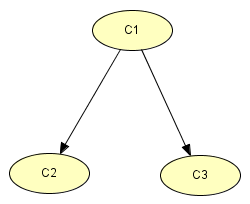
\includegraphics{Figures/BayesianPictures/BasicBayesianNetwork.png}
\caption{A simple Bayesian network}
\label{fig:basicbayesian}
\end{figure}


\subsection{Decision Trees}
Decision trees are used to represent decision problems. \ref{fig:basicdecisiontree} gives an example of a decision tree that helps investment decisions. A decision tree consists of three types of nodes: decision nodes (\ref{fig:basicdecisiontree} square boxes), chance nodes (\ref{fig:basicdecisiontree} circles) and utility nodes (\ref{fig:basicdecisiontree} triangles). The link from a decision node to a chance node is called an action, and a link from a chance node to a decision node is called a state. The idea of the decision tree is to find the path that will give us the highest utility (reward). To make a decision tree over a decision problem, every possible path of decisions have to be shown in the tree. This will create a tree that grows exponentially with the number of decision and chance nodes. Small decision problems will require big trees if not reduced. 
	
\begin{figure}[H]
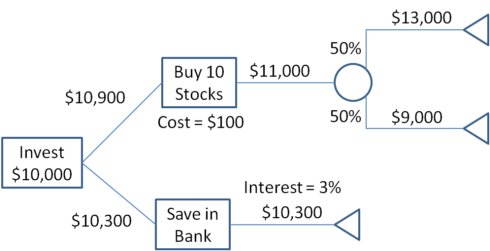
\includegraphics[scale=.5]{Figures/BayesianPictures/SimpleDecisionTree.png}
\caption{A simple decision tree \cite{sdt}}
\label{fig:basicdecisiontree}
\end{figure}

\subsection{Choice of Model}
We choose to use a Bayesian network solution for our problems because decision trees grow exponentially with the number of nodes, and 
Bayesian networks are easier to handle and manipulate.

	\section{Bayesian Network}\label{bayesian_network}
This section will describe the Bayesian networks we made to predict the enemy's spawning position, what build order they are doing and what the current 
threatlevel is. The next subsection describes the network created for predicting the enemy spawn position.




\subsection{Prediction of enemy spawn position}			 
			
The purpose of this Bayesian network is to find our opponent's spawning position. Some factors taken into account are our spawn position, enemy scouts, and time into account to help us predict this. We wanted to make this network usable on a variety of maps. Below is a visual representation of how each node is connected in the network.
%Why do we represent time as almost none, early, middle, and late?
%actual time for these times - refrace.

\insertmarginfigure{height=3in}{BayesianPictures/SpawnPrediction.png}
			{A graph of the nodes in the Spawn Prediction Bayesian network}{fig:predicting}{-3in}


\subsubsection*{EnemySpawn}
The correct state in this node is the value we are trying to discover. Ultimately, all of the evidence we collect, will be used to find this state. Most of the other variable have direct links from this node. Once we know the state of this, we are satisfied and do not need to use the network to infer more information because we do not care about predicting any of the other states.

\subsubsection*{OurSpawn}
This node is a child of EnemySpawn. We can use the values in this node to determine where the enemy does not spawn. We simply say that the enemy cannot spawn where we spawn at. At the beginning of a match we know where we spawn and can instantly put evidence on the OurSpawn node. This instantly reduces the change for our opponent to be at any other spawning location to 33\%.

\subsubsection*{EnemyNotAt(NE,SE,SW,NW)}
These nodes are used to keep track of positions we know our opponent did not spawn. Since a node can only be in one state at a time, we made four nodes that can influence the probabilities in enemy spawn. Ways we would generally get these values could be our own scouts arriving at a position and not finding our opponent.

\subsubsection*{WorkerScoutPosition} This is one of the most important variables. When we observe an enemy worker at a certain position we can influence our belief on our opponents spawn position. TimingSeen is a parent of this node. We use the information from this node to help our prediction. Just seeing an enemy at a certain position isn't enough. We need the time we see the enemy scout to help us form our beliefs. Whenever we obtain evidence on WorkerScoutPosition we will also always gather information on TimingSeen.

\subsubsection*{TimingSeen} This node is used to help us use the information from WorkerScoutPosition. It has the values: Almost None, Early, Middle, and Late. These values are the times we may see the opponent's scout. Since the values for timing depend on both map size and map layout, we purposely make the values broad.


\subsubsection*{OverlordDirection} This node is fairly simple and contributes a lot in predicting the spawn location. Since overlords are so slow, a player will be able to use the direction the overlord is coming from to predict the spawn location. By the time an overlord would have visited two bases we probably already know where the enemy's base is. This variable may seem really useful, but it only helps when fighting against zerg players. The overlord can take a while to get to even its first base, and by then we might have already needed to know where our opponent is. EnemySpawn is a parent of OverlordDirection. Once we know the direction the overlord is coming from we gain a lot of information on the enemy's spawn position.

\subsection{Build Order Prediction}
This subsection describes the Bayesian networks that was created for predicting that buildorder the enemy is doing. There are three different networks, one each for every race that the bot can encounter: Terran versus Terran, Terran versus Protoss and Terran vs Zerg.

\subsubsection{Terran versus Terran}
	This network will try to predict the following buildorders: Proxy Rush, 2 Factory Vulture Pressure, 1 Factory Expand, 1 Starport Wraith and Stim Rush. 
	Every building which is used in the buildorders are put as a node in the network. The numbers in the node names are how many of the given unit the 
	enemy have, e.g. Barracks2 means the second barracks the bot scouts. The order in which the buildings come is also modelled with the arrows, 
	e.g. the node for Factory2 points to the node for Factory1. Each of the building nodes have the states Seen and NotSeen, though Seen is only used when 
	presenting evidence, because the bot will never be able to prove that the enemy building does not exist. As the evidence is presenting the buildorder 
	probabilities rises according to how many buildings it needs have evidence on them, this gives a prediction of the given buildorders.
	
\subsubsection{Terran versus Protoss}
This model consists of six nodes, named BuildChosen, GateWay1, Nexus, Assimilator, CyberneticsCore and Gateway2. These six nodes are chosen  because they are the required buildings in order to do four will known build orders. The four build orders are TwoGate, Basic Order, 10/15 and 14 Nexus.
The two gate tactic is building two early gateways and there by making a early attack. The Basic build is a gateway at 10 supply, an assimilator at 12 and a cybernetics core at 14. The build order 10/15 is where you build a Gateway at 10 supply, an assimilator at 11 a cybernetics core at 13  and a 
another gateway at 15. The build order 14 Nexus is named so because the protoss waits until 14 supply to build a nexus as the first building. \\
As seen in the figure, there is a parent node BuildChosen this node have the four build orders as states, so by putting evidence on some of the child nodes, the bot will know the probability of the different build orders. So if the scout finds a new nexus the opponent is probably using the build order
14 Nexus. If the scout on the other hand see two gateways without cybernetics core the probability is high that it is a two gate build order. It is more unclear what the build order is if the scout see a Gateway, an assimilator and a cybernetics core. Because it could be a  

%NEED figure

\subsubsection{Terran vs Zerg}
	This network will try to predict the following buildorders: 2 Hatch Muta, 3 Hatch Muta, 3 Hatch Lurker and Early Pool Rush, 
	where Early Pool Rush is a 4pool or 5pool. Every building which is used in the buildorders are put as a node in the network. 
	The numbers in the node names are how many of the given unit the enemy have, e.g. Hatchery2 means the second hatchery the bot scouts. 
	The order in which the buildings come is also modelled with the arrows, 
	e.g. the node for Hatchery3 points to the node for Hatchery2. Each of the building nodes have the states Seen and NotSeen, 
	though Seen is only used when presenting evidence, because the bot will never be able to prove that the 
	enemy building does not exist. As the evidence is presenting the buildorder 
	probabilities rises according to how many buildings it needs have evidence on them, this gives a prediction of the given buildorders.

\subsection{Threat Level Prediction}
	This prediction is closely related to the prediction of the buildorder the enemy is doing. A buildorder have a certain time where it is effective 
	or where it hits. So determine what the current threatlevel is two nodes have to be added to each of the buildorder prediction networks, ThreatLevel 
	and Time. PUT FIGURE OF THIS HERE.

%\subsection{Conclusion of Bayesion Network}
%	We can apply Bayesion networks to the scouting and threat level prediction, by analyzing the opponent's army and build order. To calculate the predictions, we hat to take race into account. By doing this one can calculate what to expect and
%	thereby have a advantage over the opponent. In order to build the Bayesion network, one had to create the necessary nodes for spawns and scouting.
	












 

